\documentclass[conference]{IEEEtran}

\usepackage[T1]{fontenc}
\usepackage{amsmath}
\usepackage{booktabs}
\usepackage{graphicx}
\usepackage{url}
\usepackage{xspace}

% Every number in the text is a macro from this file, written by paper/make_tables.py
% from the committed files in eval_results/ and review/. Do not type numbers by hand.
% Generated by paper/make_tables.py. Do not edit by hand.
\RequirePackage{xspace}
\newcommand{\AfifteenDeltaVeight}{$-$0.07\xspace}
\newcommand{\AfifteenDeltaVnine}{+0.68\xspace}
\newcommand{\AfifteenPairs}{10\xspace}
\newcommand{\AlwaysMaps}{1\xspace}
\newcommand{\AnchorAlpha}{25\xspace}
\newcommand{\AnineBase}{5\xspace}
\newcommand{\AnineOnlyBase}{2\xspace}
\newcommand{\AnineOnlyRL}{4\xspace}
\newcommand{\AnineP}{0.69\xspace}
\newcommand{\AninePCorr}{1.00\xspace}
\newcommand{\AnineRL}{7\xspace}
\newcommand{\BaseCompl}{48.0\xspace}
\newcommand{\BaseFin}{25\xspace}
\newcommand{\BaseMapsAny}{4\xspace}
\newcommand{\BaseRecovery}{6{,}543\xspace}
\newcommand{\BaseWalls}{41\xspace}
\newcommand{\BehRuns}{13\xspace}
\newcommand{\BehStates}{11{,}608\xspace}
\newcommand{\BehVthreeNeg}{11\xspace}
\newcommand{\BehVthreeR}{$-$0.22\xspace}
\newcommand{\BehVthreeSat}{0.2\xspace}
\newcommand{\BehVthreeSteerA}{0.13\xspace}
\newcommand{\BehVtwoNeg}{8\xspace}
\newcommand{\BehVtwoR}{$-$0.14\xspace}
\newcommand{\BehVtwoSat}{0.0\xspace}
\newcommand{\BehVtwoSteerA}{0.09\xspace}
\newcommand{\BootResamples}{10{,}000\xspace}
\newcommand{\BsevenBase}{2\xspace}
\newcommand{\BsevenOnlyBase}{0\xspace}
\newcommand{\BsevenOnlyRL}{7\xspace}
\newcommand{\BsevenP}{0.016\xspace}
\newcommand{\BsevenPCorr}{0.16\xspace}
\newcommand{\BsevenRL}{9\xspace}
\newcommand{\BsevenVeight}{8\xspace}
\newcommand{\BufferEnd}{330{,}769\xspace}
\newcommand{\BufferStart}{155{,}107\xspace}
\newcommand{\CampaignFin}{27\xspace}
\newcommand{\CampaignMaps}{63\xspace}
\newcommand{\ComplDiff}{+6.7\xspace}
\newcommand{\ComplHi}{+20.0\xspace}
\newcommand{\ComplLo}{$-$1.5\xspace}
\newcommand{\CriticMaps}{6\xspace}
\newcommand{\CriticRHi}{1.00\xspace}
\newcommand{\CriticRLo}{0.89\xspace}
\newcommand{\CtwoBase}{8\xspace}
\newcommand{\CtwoOnlyBase}{7\xspace}
\newcommand{\CtwoOnlyRL}{0\xspace}
\newcommand{\CtwoP}{0.016\xspace}
\newcommand{\CtwoPCorr}{0.16\xspace}
\newcommand{\CtwoRL}{1\xspace}
\newcommand{\CtwoVeight}{3\xspace}
\newcommand{\DesignEffect}{7.2\xspace}
\newcommand{\DevBaseCompl}{95.0\xspace}
\newcommand{\DevBaseFin}{59\xspace}
\newcommand{\DevBaseWalls}{6\xspace}
\newcommand{\DevOnlyBase}{2\xspace}
\newcommand{\DevOnlyRL}{3\xspace}
\newcommand{\DevRuns}{70\xspace}
\newcommand{\DevSignP}{1.0\xspace}
\newcommand{\DevVthreeCompl}{97.4\xspace}
\newcommand{\DevVthreeFin}{60\xspace}
\newcommand{\DevVthreeWalls}{20\xspace}
\newcommand{\DevVtwoCompl}{94.4\xspace}
\newcommand{\DevVtwoFin}{60\xspace}
\newcommand{\ESS}{14\xspace}
\newcommand{\ExploreSigma}{0.2\xspace}
\newcommand{\FinDiff}{+2.0\xspace}
\newcommand{\FinHi}{+23.0\xspace}
\newcommand{\FinLo}{$-$19.0\xspace}
\newcommand{\FloorMaps}{6\xspace}
\newcommand{\FloorMapsP}{0.031\xspace}
\newcommand{\FreshMaps}{26\xspace}
\newcommand{\FreshMapsNonBlack}{23\xspace}
\newcommand{\GameSpeed}{10\xspace}
\newcommand{\Gravity}{24.87\xspace}
\newcommand{\GravityMaps}{53\xspace}
\newcommand{\GravityNewRatio}{1.01\xspace}
\newcommand{\GravityOldRatio}{0.80\xspace}
\newcommand{\GripAUC}{0.754\xspace}
\newcommand{\GripAUCDemand}{0.755\xspace}
\newcommand{\GripAUCSpeed}{0.708\xspace}
\newcommand{\GripBaseRate}{5.7\xspace}
\newcommand{\GripDemandCoef}{0.132\xspace}
\newcommand{\GripIntercept}{-12.0\xspace}
\newcommand{\GripMaps}{54\xspace}
\newcommand{\GripRisk}{0.2\xspace}
\newcommand{\GripSamples}{32{,}210\xspace}
\newcommand{\GripSpeedCoef}{0.108\xspace}
\newcommand{\ICC}{0.69\xspace}
\newcommand{\IQNFirstFrames}{3.18M\xspace}
\newcommand{\IQNFirstOther}{0\xspace}
\newcommand{\IQNHockBest}{54.06\xspace}
\newcommand{\IQNHockFin}{5\xspace}
\newcommand{\IQNHockRuns}{10\xspace}
\newcommand{\IQNLastAthree}{8\xspace}
\newcommand{\IQNLastFrames}{10.64M\xspace}
\newcommand{\IQNLastOther}{8\xspace}
\newcommand{\IQNOtherMaps}{5\xspace}
\newcommand{\IQNOtherRuns}{50\xspace}
\newcommand{\ImpactDrop}{4\xspace}
\newcommand{\InformativeMaps}{3\xspace}
\newcommand{\LateralAUC}{0.76\xspace}
\newcommand{\LidarAUC}{0.62\xspace}
\newcommand{\LidarHitPct}{56\xspace}
\newcommand{\LidarOrdPct}{10\xspace}
\newcommand{\MapP}{1.0\xspace}
\newcommand{\MapPFloor}{0.25\xspace}
\newcommand{\NDev}{7\xspace}
\newcommand{\NOfflineTrain}{53\xspace}
\newcommand{\NRLTrain}{6\xspace}
\newcommand{\NRays}{13\xspace}
\newcommand{\NTest}{10\xspace}
\newcommand{\NeverMaps}{6\xspace}
\newcommand{\NoiseHold}{10\xspace}
\newcommand{\NoiseSeed}{0\xspace}
\newcommand{\NoiseSigma}{0.05\xspace}
\newcommand{\ObsSize}{39\xspace}
\newcommand{\PairsBoth}{16\xspace}
\newcommand{\PairsNeither}{64\xspace}
\newcommand{\PairsOnlyBase}{9\xspace}
\newcommand{\PairsOnlyRL}{11\xspace}
\newcommand{\PowerHi}{0.90\xspace}
\newcommand{\PowerHiGain}{20.5\xspace}
\newcommand{\PowerHiOR}{6\xspace}
\newcommand{\PowerLo}{0.64\xspace}
\newcommand{\PowerLoGain}{14.9\xspace}
\newcommand{\PowerLoOR}{4\xspace}
\newcommand{\PowerSims}{2{,}000\xspace}
\newcommand{\RayRange}{60\xspace}
\newcommand{\ReanalysisSeed}{20261117\xspace}
\newcommand{\RecoveryDropPct}{23\xspace}
\newcommand{\ResSpeed}{8\xspace}
\newcommand{\ResSteer}{0.25\xspace}
\newcommand{\RunsPerMap}{10\xspace}
\newcommand{\SignP}{0.82\xspace}
\newcommand{\SingleRecDropPct}{42\xspace}
\newcommand{\SingleVeightFin}{4\xspace}
\newcommand{\SingleVeightRec}{431\xspace}
\newcommand{\SingleVsevenFin}{2\xspace}
\newcommand{\SingleVsevenRec}{747\xspace}
\newcommand{\SingleWallsVfive}{11\xspace}
\newcommand{\SingleWallsVfour}{2\xspace}
\newcommand{\SingleWallsVsix}{2\xspace}
\newcommand{\SpeedCVr}{0.81\xspace}
\newcommand{\SpeedFeatures}{18\xspace}
\newcommand{\SpeedHandr}{0.33\xspace}
\newcommand{\SpeedHidden}{64\xspace}
\newcommand{\SpeedLinr}{0.57\xspace}
\newcommand{\SplitSeed}{20261112\xspace}
\newcommand{\StackEraOneMapsFin}{5\xspace}
\newcommand{\StepMs}{50\xspace}
\newcommand{\StuckCutoff}{6\xspace}
\newcommand{\TDGamma}{0.99\xspace}
\newcommand{\TDHidden}{256\xspace}
\newcommand{\TestRuns}{100\xspace}
\newcommand{\TimeRatioHi}{1.63\xspace}
\newcommand{\TimeRatioLo}{1.44\xspace}
\newcommand{\TopSpeed}{70\xspace}
\newcommand{\TrainEpisodes}{200\xspace}
\newcommand{\TrainExtraMaps}{14\xspace}
\newcommand{\TrainMaps}{20\xspace}
\newcommand{\TrainNoise}{0.05\xspace}
\newcommand{\TrainNoiseSeed}{1000\xspace}
\newcommand{\TrainPoolSeed}{20261113\xspace}
\newcommand{\UnchangedMaps}{7\xspace}
\newcommand{\VeightFin}{26\xspace}
\newcommand{\VeightOnlyBase}{9\xspace}
\newcommand{\VeightOnlyRL}{10\xspace}
\newcommand{\VeightSignP}{1.0\xspace}
\newcommand{\VnineCompl}{54.7\xspace}
\newcommand{\VnineFin}{27\xspace}
\newcommand{\VnineRecovery}{5{,}043\xspace}
\newcommand{\VnineWalls}{32\xspace}
\newcommand{\WallsDropPct}{22\xspace}
\newcommand{\ZeroSame}{760\xspace}
\newcommand{\ZeroSteps}{760\xspace}

\xspaceaddexceptions{\, \%}

\newcommand{\vseven}{v7\xspace}
\newcommand{\veight}{v8\_rl\xspace}
\newcommand{\vnine}{v9\_rl\xspace}

\begin{document}

\title{A Classical Driving Stack Generalises Where End-to-End RL Did Not;\\
a Residual Policy on Top Mostly Reshuffles Which Tracks Finish}

\author{\IEEEauthorblockN{Stormy-1}
\IEEEauthorblockA{Independent project\\
\url{https://github.com/Stormy-1/linesight-trackmania-rl}}}

\maketitle

\begin{abstract}
We report a null result for residual reinforcement learning in a racing simulator, and the evaluation
design that exposes it. An end-to-end IQN agent trained from pixels in TrackMania Nations Forever learned its
training track but finished \IQNLastOther of \IQNOtherRuns greedy runs on \IQNOtherMaps other tracks, all on one of them.
A classical stack (map matching to the track's official reference lap, a speed profile, pure pursuit and
safety layers) whose hand-set constants are replaced by small learned models finished \CampaignFin of \CampaignMaps campaign tracks in single runs. On
\NTest held-out tracks, each driven \RunsPerMap times under seeded steering noise, it finishes \BaseFin of
\TestRuns runs. Adding a bounded residual TD3 policy gives \VnineFin of \TestRuns (paired sign test
$p=\SignP$; sign-flip test over tracks $p=\MapP$). The policy improves one track, damages another,
and leaves \UnchangedMaps of the \NTest unchanged. Finishing is strongly clustered by track
(intraclass correlation \ICC), so the
\TestRuns runs carry about as much information as \ESS independent ones, and only a gain of roughly
\PowerLoGain to \PowerHiGain points of finish rate could have been detected; smaller effects are not ruled
out. More runs per track would not change that; more tracks would.
\end{abstract}

\section{Introduction}

Racing games are a common testbed for deep reinforcement learning (RL) because they offer fast, cheap and
exactly repeatable driving \cite{TODO-gt-sophy}. They are also a place where a classical robotics pipeline is
easy to build: the simulator reports the exact pose, and every track ships with a reference lap. This paper
compares the two on one game, TrackMania Nations Forever, and then asks whether RL helps when it is restricted
to correcting the classical pipeline rather than replacing it.

The project ran in two eras. In the first, an Implicit Quantile Network (IQN) \cite{dabney2018iqn} from the
Linesight framework \cite{linesight} learned a single track from pixels and telemetry. It did not transfer
(Table~\ref{tab:generalisation}). In the second, a classical sense, plan and act loop drove the car, small
learned models replaced its hand-set constants, and a residual TD3 policy
\cite{fujimoto2018td3,silver2018residual,johannink2019residual} added bounded corrections on top.

Our position is that the classical stack generalised where end-to-end RL did not, and that the residual policy
mostly reshuffles which tracks finish. The second half of that claim rests on an evaluation built to tell a
real effect from run-to-run luck, and on an honest account of how little ten tracks can resolve. The
contributions are:
\begin{itemize}
\item a classical driving stack whose speed limit, grip limit, gravity constant and obstacle shapes are
  learned or measured from data, with every model validated on tracks it was not fitted on
  (Section~\ref{sec:method});
\item a paired, seeded evaluation of a residual RL policy on held-out tracks, with the policy chosen for its
  single test look by a rule fixed in advance (Section~\ref{sec:protocol});
\item a reanalysis with the track as the unit, which shows the residual effect is a null and quantifies the
  smallest effect this design could have detected (Section~\ref{sec:results}).
\end{itemize}

\section{Related Work}

\textbf{End-to-end RL for driving games.} Deep RL agents have reached expert level in racing simulators when
trained at scale \cite{TODO-gt-sophy}. Distributional value methods such as IQN \cite{dabney2018iqn} are the
basis of Linesight \cite{linesight}, an open-source agent for TrackMania that learns from screen pixels.
Overfitting to training environments is a known failure of deep RL \cite{TODO-rl-generalisation}; our era-1
agent is one more instance of it.

\textbf{Classical vehicle control.} Pure pursuit \cite{coulter1992purepursuit} steers toward a point on a
reference path a fixed distance ahead. Autonomous racing more often uses optimisation-based planning and
model predictive control \cite{TODO-racing-survey,TODO-mpc-racing}. We use pure pursuit because it has few
parameters and none of them is specific to a track.

\textbf{Residual RL.} Residual policy learning \cite{silver2018residual} and residual RL for robot control
\cite{johannink2019residual} learn a correction that is added to a fixed controller, so learning starts from a
working policy. We use TD3 \cite{fujimoto2018td3} as the learner and the behaviour-cloning anchor of TD3+BC
\cite{fujimoto2021td3bc}, applied here toward the zero correction rather than toward logged actions.

\textbf{Evaluation.} Reported gains in deep RL are often within run-to-run variance
\cite{TODO-rl-statistics}. When outcomes are clustered, the effective sample size falls by the design effect
\cite{TODO-design-effect}. Our map-level analysis applies that correction to a driving benchmark.

\section{Method}
\label{sec:method}

\subsection{Classical stack}

The game runs at \GameSpeed{}$\times$ real time and the controller acts every \StepMs\,ms of game time through
TMInterface \cite{TODO-tminterface}, which reports the exact pose. Localisation is therefore free; the hard
parts are the reference line, the speed plan and control through digital keys.

\textbf{Line and map matching.} Each campaign track ships an official replay of the author's lap. Its ghost is
resampled into a reference line, and the car is projected onto it every step with a search window around the
previous match, so the projection cannot jump to a crossing section of track.

\textbf{Speed profile.} A target speed is computed for every point of the line: a corner limit, a backward
braking pass, and a speed floor over jumps derived from the reference car's ballistic flight.

\textbf{Control and safety.} Pure pursuit \cite{coulter1992purepursuit} steers toward a lookahead point, with
a steering cap that shrinks at high speed. Throttle and brake track the target speed. A sigma-delta adapter
maps the continuous commands onto the game's digital keys. Safety layers take over when the car leaves the
line (recovery), stalls (reverse) or slides (slip guard).

\subsection{Learned components}

Four hand-set quantities were replaced by models fitted to data, each validated by track
(Table~\ref{tab:models}).

\textbf{Speed model.} An MLP with \SpeedHidden-unit hidden layers maps \SpeedFeatures geometry features of the
line (curvature ahead and behind, slopes, crests, jump features) to the speed of the official replays. In
cross-validation with folds by track it reaches $r=\SpeedCVr$, against $\SpeedLinr$ for a linear model on the
same features and $\SpeedHandr$ for the hand rule it replaced.

\textbf{Grip limit.} The pro's speed is not this car's speed: pros drift through corners the controller
cannot hold. A logistic model, fitted on \GripSamples cornering steps of our own driving on \GripMaps
non-test tracks, predicts whether the car runs wide (base rate \GripBaseRate\%):
$\operatorname{logit} P = \GripIntercept + \GripDemandCoef\, v^2|\kappa| + \GripSpeedCoef\, v$.
Solving for $v$ at risk $p=\GripRisk$, chosen on dev tracks, caps the corner speed. The speed term changes the shape of the limit
but not its ranking power: the lateral demand $v^2|\kappa|$ alone has the same leave-one-map-out AUC.

\textbf{Gravity.} Steady free fall in the ghosts of \GravityMaps tracks gives
$g=\Gravity$\,m/s$^2$ (\texttt{gravity\_measurement.json}). With it, the jump detector's required speed
matches the pro's measured speed at a median ratio of \GravityNewRatio, against \GravityOldRatio with the
earlier guessed value.

\textbf{Virtual lidar.} Obstacle shapes are learned per block type, not per track, from the cells that pro
ghosts never entered, and \NRays rays are cast over them out to \RayRange\,m. As a crash warning on its own
it is weak (AUC \LidarAUC, against \LateralAUC for lateral error), so it is used only as an observation for
the residual policy.

\begin{table}[t]
\caption{Learned-model validation. All splits are by track. LOMO: leave one map out.}
\label{tab:models}
\centering
\resizebox{\columnwidth}{!}{\begin{tabular}{@{}llll@{}}
\toprule
Model & Validation & Result & Reference \\
\midrule
Speed MLP & CV by map & $r$ 0.81, MAE 11.7 & hand rule $r$ 0.33, MAE 34.1 \\
Speed MLP & test, once & $r$ 0.84, MAE 10.3 & hand rule $r$ 0.21, MAE 31.1 \\
Grip logistic & LOMO, 54 maps & AUC 0.754 & $v^2|\kappa|$ alone 0.755 \\
Grip logistic & test, once & AUC 0.84 &  \\
Virtual lidar & LOMO, 43 hits & contact at 56\% of hits & 10\% of other steps \\
Gravity & 2{,}328 samples & 24.87 m/s$^2$ & IQR 24.55--25.25 \\
\bottomrule
\end{tabular}
}
\end{table}

\subsection{Residual policy}

The residual policy outputs $a\in[-1,1]^2$, scaled to a steering change of at most \ResSteer of full lock
and a target-speed change of at most \ResSpeed\,m/s, both added before the safety layers. It is gated off
while a safety layer owns the car. Its \ObsSize-dimensional observation holds the track-relative state, the
base command, lookahead geometry, the \NRays lidar rays and wheel contact, all divided by fixed physical
scales and with no track identity. The reward is progress minus penalties for impacts, recovery steps,
getting stuck and action magnitude.

TD3 \cite{fujimoto2018td3} trains it with two-layer, \TDHidden-unit networks and $\gamma=\TDGamma$. Four
choices make training start from the base stack. The actor's output layer is initialised to zero, so the
untrained policy drives exactly like the base: in a live check, \ZeroSame of \ZeroSteps steps had identical
commands. The critics were first fitted to the base stack's own runs on the \CriticMaps training tracks,
reaching $r=\CriticRLo$ to \CriticRHi between predicted and realised return. The actor loss carries a TD3+BC
style anchor \cite{fujimoto2021td3bc} toward zero action; at the first strength tried, in a first policy (td3\_v1), the actor did not
move, and the final weight is \AnchorAlpha (\texttt{td3\_v3/train\_config.json}). Exploration noise
($\sigma=\ExploreSigma$) is held for \NoiseHold steps so that a correction lasts long enough to survive the
key adapter. These choices are supported by training-time diagnostics, not by ablations on held-out tracks.

Two policies reach the test set. td3\_v2 trained on the \NRLTrain training tracks without perturbation.
td3\_v3 was initialised from td3\_v2's weights and trained for \TrainEpisodes episodes on \TrainMaps tracks
(the \NRLTrain plus \TrainExtraMaps drawn by a fixed rule with seed \TrainPoolSeed, never dev or test), with
steering noise $\sigma=\TrainNoise$ on a seed different from evaluation. Its replay buffer was seeded with
td3\_v1 and td3\_v2's episodes; it held \BufferStart transitions after the first episode and \BufferEnd at
the end.

\section{Experimental Protocol}
\label{sec:protocol}

\textbf{Split.} The campaign tracks were split once, with seed \SplitSeed: \NDev dev tracks for every design
choice, \NTest held-out test tracks drawn from four difficulty tiers, \NRLTrain RL training tracks, and the
\NOfflineTrain non-test official replays as offline data (\texttt{maps/map\_split.json}). Every test run
receives identical arguments; the report script refuses any run with a per-track speed cap.

\textbf{Paired noisy runs.} A run is deterministic without noise, so a single run per track measures one
draw of a knife-edge outcome. Each version was therefore driven \RunsPerMap times per test track with
Gaussian noise ($\sigma=\NoiseSigma$) added to the steering sent to the keys, seed \NoiseSeed. Run $k$
receives the same noise stream in every version, which pairs runs across versions. A run ends at the finish,
after \StuckCutoff\,s without progress, or at a time limit. The settings were fixed before any result was
seen, and checked only on one dev track.

\textbf{Versions.} \vseven is the classical stack with the learned models. \veight adds td3\_v2 and \vnine
adds td3\_v3. td3\_v3 received its test look only because it passed a rule written before its dev runs: it
had to finish more dev runs than both \vseven and td3\_v2, with ties broken by mean completion. Under the
same protocol on dev it finished \DevVthreeFin of \DevRuns runs, against \DevBaseFin for the base and
\DevVtwoFin for td3\_v2, with mean completion \DevVthreeCompl\% against \DevVtwoCompl\%
(\texttt{dev\_robustness\_*.json}). The difference from the base is itself within noise
($\DevOnlyBase$ against $\DevOnlyRL$ discordant runs, $p=\DevSignP$), and td3\_v3 hit walls more often on dev
(\DevVthreeWalls against \DevBaseWalls).

\textbf{Metrics and tests.} Finish rate is the primary metric. Mean completion, wall hits and recovery steps
are secondary. Contacts are inferred, not reported by the game: an impact is a speed drop of more than
\ImpactDrop\,m/s in one step, and impacts are classified as landings, bumps or wall hits from the trajectory.
We report the exact sign test over the \TestRuns paired runs, then repeat the analysis with the track as the
unit: an exact sign-flip test on the per-track change in finishes, and a cluster bootstrap over tracks
(\BootResamples resamples, seed \ReanalysisSeed; \texttt{scripts/reanalyze\_clustered.py}).

\section{Results}
\label{sec:results}

\subsection{Generalisation of the two eras}

Table~\ref{tab:generalisation} compares the eras. The IQN agent finished \IQNHockFin of \IQNHockRuns greedy
runs on its training track, with a best time of \IQNHockBest\,s, but \IQNFirstOther of \IQNOtherRuns on \IQNOtherMaps
other campaign tracks at \IQNFirstFrames frames and \IQNLastOther at \IQNLastFrames, all \IQNLastAthree on a
single track (\texttt{benchmark\_20261014\_190540.csv}). The classical stack, before any learned component,
finished all \StackEraOneMapsFin of those tracks and \CampaignFin of \CampaignMaps campaign tracks in one run
each. The finish count falls with difficulty tier, from White to Black.

\begin{table}[t]
\caption{Generalisation. Classical stack (v3b, no learned components) on the campaign, one run per track,
and the era-1 IQN agent, \IQNHockRuns greedy runs per track. ``Other maps'' are A01, A03, A05, A07 and A11.}
\label{tab:generalisation}
\centering
\footnotesize
\begin{tabular}{@{}llr@{}}
\toprule
Agent & Maps & Finished \\
\midrule
Stack (v3b), campaign & White & 12/15 \\
Stack (v3b), campaign & Green & 9/15 \\
Stack (v3b), campaign & Blue & 4/15 \\
Stack (v3b), campaign & Red & 2/15 \\
Stack (v3b), campaign & Black & 0/3 \\
Stack (v3b), campaign & all & 27/63 \\
IQN 3.18M, training map & Hock. & 4/10 \\
IQN 3.18M, other maps & 5 maps & 0/50 \\
IQN 10.64M, training map & Hock. & 5/10 \\
IQN 10.64M, other maps & 5 maps & 8/50 \\
\bottomrule
\end{tabular}

\end{table}

The comparison is not symmetric. The stack uses the official replay of every track as its reference line,
which the IQN agent never saw, and the stack was developed on a handful of the campaign tracks. It shows that
a pipeline with no track-specific parameters transfers; it does not show that the stack is a better driver
where both work. Finished tracks take \TimeRatioLo to \TimeRatioHi times the pro's time
(Table~\ref{tab:history}).

\subsection{Residual RL on held-out tracks}

Table~\ref{tab:robustness} gives the paired noisy evaluation. The base stack finishes \BaseFin of \TestRuns
runs; td3\_v2 finishes \VeightFin and td3\_v3 \VnineFin. Against the base, td3\_v3 has \PairsBoth runs
finished by both, \PairsOnlyBase by the base only, \PairsOnlyRL by the residual only and \PairsNeither by
neither, an exact sign test $p=\SignP$. td3\_v2 gives \VeightOnlyBase against \VeightOnlyRL
($p=\VeightSignP$).

The secondary metrics move in the residual's favour: mean completion rises from \BaseCompl\% to
\VnineCompl\%, wall hits fall \WallsDropPct\% and recovery steps \RecoveryDropPct\%. The completion change is not
distinguishable from zero once tracks are the unit (Table~\ref{tab:maplevel}), and the wall and recovery counts were not tested at the track level. Lap times barely change: on
A15, where every run finishes, the paired median change is \AfifteenDeltaVeight\,s for td3\_v2 and
\AfifteenDeltaVnine\,s for td3\_v3 over \AfifteenPairs pairs.

\begin{table}[t]
\caption{Held-out tracks, \RunsPerMap paired runs per track under steering noise. Finishes out of \RunsPerMap; mean
completion; discordant pairs (finished by \vseven only / by \vnine only).}
\label{tab:robustness}
\centering
\resizebox{\columnwidth}{!}{\begin{tabular}{@{}llrrrrrc@{}}
\toprule
Map & Tier & v7 & v8\_rl & v9\_rl & \multicolumn{2}{c}{Compl.\ (\%)} & Disc. \\
 & & \multicolumn{3}{c}{finished / 10} & v7 & v9\_rl & v7 / v9\_rl \\
\midrule
A09 & White & 5 & 5 & 7 & 81.2 & 89.9 & 2 / 4 \\
A15 & White & 10 & 10 & 10 & 100.0 & 100.0 & 0 / 0 \\
B04 & Green & 0 & 0 & 0 & 54.2 & 54.2 & 0 / 0 \\
B07 & Green & 2 & 8 & 9 & 30.3 & 91.3 & 0 / 7 \\
B13 & Green & 0 & 0 & 0 & 8.3 & 8.3 & 0 / 0 \\
C02 & Blue & 8 & 3 & 1 & 99.0 & 88.3 & 7 / 0 \\
C10 & Blue & 0 & 0 & 0 & 45.0 & 45.0 & 0 / 0 \\
C13 & Blue & 0 & 0 & 0 & 7.9 & 7.9 & 0 / 0 \\
D04 & Red & 0 & 0 & 0 & 9.9 & 9.8 & 0 / 0 \\
D07 & Red & 0 & 0 & 0 & 43.9 & 52.1 & 0 / 0 \\
\midrule
Total & & 25 & 26 & 27 & 48.0 & 54.7 & 9 / 11 \\
Walls & & 41 & 39 & 32 & & & \\
Recovery & & 6{,}543 & 6{,}516 & 5{,}043 & & & \\
\bottomrule
\end{tabular}
}
\end{table}

The total hides a trade. Both residual policies improve B07 (\BsevenBase/\RunsPerMap for the base, \BsevenVeight/\RunsPerMap for
td3\_v2, \BsevenRL/\RunsPerMap for td3\_v3) and damage C02 (\CtwoBase/\RunsPerMap, \CtwoVeight/\RunsPerMap, \CtwoRL/\RunsPerMap). For td3\_v3
both tracks split \BsevenOnlyRL pairs to \BsevenOnlyBase, $p=\BsevenP$ each, or about \BsevenPCorr after a
Bonferroni correction for \NTest tracks. A09 moves from \AnineBase to \AnineRL finishes ($p=\AnineP$). The other
\UnchangedMaps tracks give identical finish counts for the base and td3\_v3. The policy therefore changes which tracks finish
more than how many.

\subsection{The track as the unit}

The sign test over runs assumes \TestRuns independent pairs. They are not independent: runs on one track share
its geometry, and the noise only nudges the car around the same knife-edge events. The intraclass
correlation of finishing in the base version is \ICC, a design effect of \DesignEffect, so the \TestRuns runs
carry about the information of \ESS independent ones.

\begin{table}[t]
\caption{Track-level analysis against \vseven. $p$: exact sign-flip test over tracks. Floor: smallest $p$
this design could produce given how many tracks changed. $\Delta$: change in points, cluster bootstrap over
tracks, 95\% interval.}
\label{tab:maplevel}
\centering
\resizebox{\columnwidth}{!}{\begin{tabular}{@{}lrrcrc@{}}
\toprule
vs v7 & $p_{\mathrm{fin}}$ & floor & $\Delta$ finish rate & $p_{\mathrm{compl}}$ & $\Delta$ completion \\
\midrule
v8\_rl & 1.0 & 0.50 & +1.0 [$-$15.0, +18.0] & 0.55 & +4.9 [$-$3.0, +16.7] \\
v9\_rl & 1.0 & 0.25 & +2.0 [$-$19.0, +23.0] & 0.48 & +6.7 [$-$1.5, +20.0] \\
\bottomrule
\end{tabular}
}
\end{table}

\begin{figure}[t]
\centering
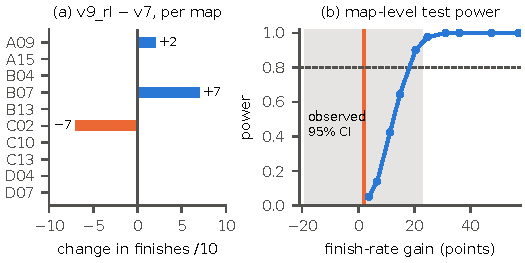
\includegraphics[width=\columnwidth]{generated/fig_maps_power.pdf}
\caption{(a) Change in finishes per held-out track, td3\_v3 against the base; only three tracks move.
(b) Power of the track-level sign-flip test at $\alpha=0.05$ against the expected gain in finish rate
(\PowerSims simulated studies per point), with the observed change and its 95\% bootstrap interval.}
\label{fig:power}
\end{figure}

With the track as the unit there is nothing to detect (Table~\ref{tab:maplevel}, Fig.~\ref{fig:power}a).
\NeverMaps tracks never finish in any version and \AlwaysMaps always does, so only \InformativeMaps tracks
contribute a discordant pair. The sign-flip test on the change in finishes gives $p=\MapP$ for both
policies. Even if every changed track had moved in the residual's favour, \InformativeMaps tracks could give
at best $p=\MapPFloor$; reaching $p<0.05$ needs at least \FloorMaps tracks moving in one direction. The
bootstrap interval for td3\_v3's change in finish rate runs from \FinLo to \FinHi points, and for mean
completion from \ComplLo to \ComplHi.

A power simulation makes the limit concrete (Fig.~\ref{fig:power}b). Multiplying every track's finish odds by
a common odds ratio, the track-level test reaches power \PowerLo at an odds ratio of \PowerLoOR (an expected
gain of \PowerLoGain points) and \PowerHi at \PowerHiOR (\PowerHiGain points). The observed change is
\FinDiff points. The simulation assumes a common odds ratio on every track and independent runs, and smooths
the base rates so that tracks at 0 or \RunsPerMap finishes can move. That is optimistic: the tracks that never
finish stall early on geometry that a bounded correction is unlikely to change. Because the information sits
in the tracks, not the runs, more runs per track would not lower this threshold.

\subsection{Why single runs misled}

Before the paired evaluation, each version was driven once per test track (Table~\ref{tab:history}). In that
history the residual looked like a clear gain: \SingleVeightFin of \NTest tracks against \SingleVsevenFin,
and recovery steps down \SingleRecDropPct\%. Under noise, the same base finishes A09 \AnineBase times in \RunsPerMap
and C02 \CtwoBase times in \RunsPerMap, so a single run on those tracks is close to a coin flip. That sensitivity
accounts for the single-run gain, and the churn of the finished set from v4 to \vseven is consistent with
it. The history also shows the learned models trading one failure for another: the speed model alone raised
wall hits from \SingleWallsVfour to \SingleWallsVfive, and the grip limit brought them back to \SingleWallsVsix.

\begin{table}[t]
\caption{Single deterministic run per held-out track, in the order the components were added. $t/t_{\mathrm{pro}}$:
median finish time over the pro's, over finished tracks.}
\label{tab:history}
\centering
\footnotesize
\begin{tabular}{@{}llrrrrr@{}}
\toprule
Ver. & Change & Fin. & Compl.\,\% & $t/t_{\mathrm{pro}}$ & Walls & Recov. \\
\midrule
v4 & classical stack & 3/10 & 57.9 & 1.60 & 2 & 529 \\
v5 & + learned speed & 3/10 & 52.3 & 1.63 & 11 & 734 \\
v6 & + grip limit & 2/10 & 54.0 & 1.50 & 2 & 677 \\
v7 & + measured $g$ & 2/10 & 46.2 & 1.44 & 1 & 747 \\
v8\_rl & + residual TD3 & 4/10 & 58.1 & 1.50 & 1 & 431 \\
\bottomrule
\end{tabular}

\end{table}

\subsection{What the residual does}

On \BehStates states from dev and training runs (\texttt{td3\_v3\_behaviour.json}), td3\_v3's mean steering
correction is \BehVthreeSteerA of full scale, it saturates in \BehVthreeSat\% of states, and its steering
correlates with the sine of the heading error at $r={}$\BehVthreeR, negative on \BehVthreeNeg of \BehRuns runs.
td3\_v2 shows the same sign more weakly ($r={}$\BehVtwoR, \BehVtwoNeg of \BehRuns). This is a weak damping
tendency on top of pure pursuit. It is small enough that it can only change outcomes where the base stack is
already marginal, which matches the tracks it moves: B07 and C02 both finish under some noise draws for at
least one version. The causes on C02 were not studied, since that would mean designing against test-track
logs.

\section{Limitations}
\label{sec:limitations}

\textbf{The test set has been looked at seven times.} The looks were the single runs of v4, v5, v6, \vseven
and \veight, the paired re-evaluation of \vseven and \veight, and the paired evaluation of \vnine. No
parameter was tuned on a test track, but after v6 the failure logs of two test tracks (A09 and C02, both at
jumps) were studied, and that study led to the gravity measurement in \vseven. The fix is a physics constant
measured on non-test ghosts, not a per-track change. It is still leakage: the test set steered what was
built next. The \vseven numbers are therefore not fully held out, and a new claim would need a fresh set of
tracks. The rule that admitted td3\_v3 to its look was written before its dev runs, but only in project notes with
no committed timestamp, and the margin by which td3\_v3 passed it is within noise.

\textbf{Collisions are inferred.} The game reports no contacts. Wall hits and landings come from a speed
drop above \ImpactDrop\,m/s in one step and a trajectory classifier. Wall-hit counts, the reward's impact
penalty and the lidar validation all inherit its errors, which have not been measured against ground truth.

\textbf{The campaign result is a single run per track.} The \CampaignFin of \CampaignMaps figure uses one
deterministic run per track, and the stack had been developed on five of those tracks (a count from the project record,
\texttt{RESULTS.md}, not from a result file). Given the run-to-run
sensitivity shown above, the per-tier counts in Table~\ref{tab:generalisation} could move by several tracks
under noise.

\textbf{The era comparison is not controlled.} The stack is given each track's official reference lap,
a demonstration the IQN agent never had. The IQN agent was trained on a single track, and it was evaluated
on \IQNOtherMaps tracks against the stack's \CampaignMaps. The comparison shows that a pipeline without
track-specific parameters transfers when given a reference lap; it does not show that end-to-end RL with
multi-track training and the same information would fail.

\textbf{Results are simulator-only.} TrackMania has deterministic physics, exact pose and a reference lap for
every track. None of the results says anything about a physical car, where localisation and the vehicle model
are the hard parts \cite{TODO-sim2real}. Re-driving any run needs the game, and the learned models can only
be refitted from the game's own replay files, which are not redistributable.

\textbf{Ten test tracks are too few.} Only \InformativeMaps of the \NTest tracks change between versions, so
every test of the residual rests on \InformativeMaps clusters. The design can detect a gain of roughly \PowerLoGain to
\PowerHiGain points of finish rate and no smaller one. A residual effect of a few points, which the secondary
metrics hint at, is out of reach. The per-track B07 and C02 effects are large within each track, but whether
such trades generalise to other tracks is unknown.

\textbf{The two policies are not independent replications.} td3\_v3 was initialised from td3\_v2's weights,
its buffer held td3\_v2's episodes, and both were evaluated on the same noise seed. Their agreement on B07 and
C02 shows the trade is stable within one policy lineage under these noise draws. It does not show that an
independently trained policy would make the same trade. Likewise, the change in behaviour from td3\_v2 to
td3\_v3 coincides with more tracks and training noise, but td3\_v3 also had more episodes and a different
start, so its cause is not isolated.

\textbf{The car is slow.} Finished tracks take \TimeRatioLo to \TimeRatioHi times the pro's time. The
residual was evaluated against a weak base, and it is possible that a correction matters more, or less, for
a faster one.

\section{Conclusion}

On this benchmark a classical stack with learned constants transferred to unseen tracks and an end-to-end
agent did not. A bounded residual RL policy on top of that stack did not change how many held-out runs
finish; it moved the finishes from one track to another. The paired, track-level evaluation is what made this
visible, and it also bounds the claim: ten tracks cannot resolve an effect below about \PowerLoGain points.
The next experiment follows from the limitations. It needs a policy trained from a fresh initialisation and
buffer, evaluated on a new noise seed and on more tracks. The campaign still holds \FreshMaps tracks
(\FreshMapsNonBlack outside the hardest tier) never used for dev, test or RL training. They are fresh for the
residual policy and for design choices, though not for the learned models, whose fitting data include them.

\bibliographystyle{IEEEtran}
\bibliography{refs}

\end{document}
